
\documentclass{article}

\usepackage{amsmath}
\usepackage{amssymb}
\usepackage{graphicx}
\usepackage{tikz}
\usetikzlibrary{arrows}
\usepackage{verbatim}
%\usepackage{sfmath}
\usepackage{psfrag}
\usepackage{here} 
\usepackage{hyperref}
\usepackage{xcolor}
\usepackage{tcolorbox}

\title{Práctica 2}
\author{Javier Izquierdo Hernández}
\date{\today}
%\textheight=24cm

%\renewcommand\sfdefault{phv}     %use helvetica for sans serif
\renewcommand{\familydefault}{\sfdefault}
\renewcommand{\familydefault}{cmss}

\begin{document}
	\begin{titlepage}
		\centering
		{
\includegraphics[width=0.3\textwidth]{figures/logo}\par}
		\vspace{1cm}
		{\bfseries\LARGE Universidad Rey Juan Carlos \par}
		\vspace{1cm}
		{\scshape\Large E.T.S. Ingeniería de Telecomunicación \par}
		\vspace{3cm}
		{\scshape\Huge Ingeniería de Control \par}
		\vspace{3cm}
		{\itshape\Large Práctica 2 \par}
		\vfill
		{\Large Autor: \par}
		{\Large Javier Izquierdo Hernández \par}
		\vfill
		{\Large \today \par}
	\end{titlepage}
	\begin{center}
		{\huge \bf Práctica 1}
	\end{center}


Consider the simplified planar model of the control system for self balancing of a motorcycle represented in Figure~\ref{fig:figure_1}, in which the motorcycle is represented by a bar that rotates around point $\mathbf{b}$. 
Points $\mathbf{c}_1$ and  $\mathbf{c}_2$ are the positions of the centers of mass of the motorcycle and the reaction wheel, respectively. 
The control system is composed of an actuated reaction wheel, which rotates around point $\mathbf{c}_2$. A motor controls the rotation of the reaction wheel applying a torque $\tau$, which is the only input of the control system. Angles $q_1$, $q_2$ and their time derivatives are the state variables of the system.  





\begin{figure}[h]
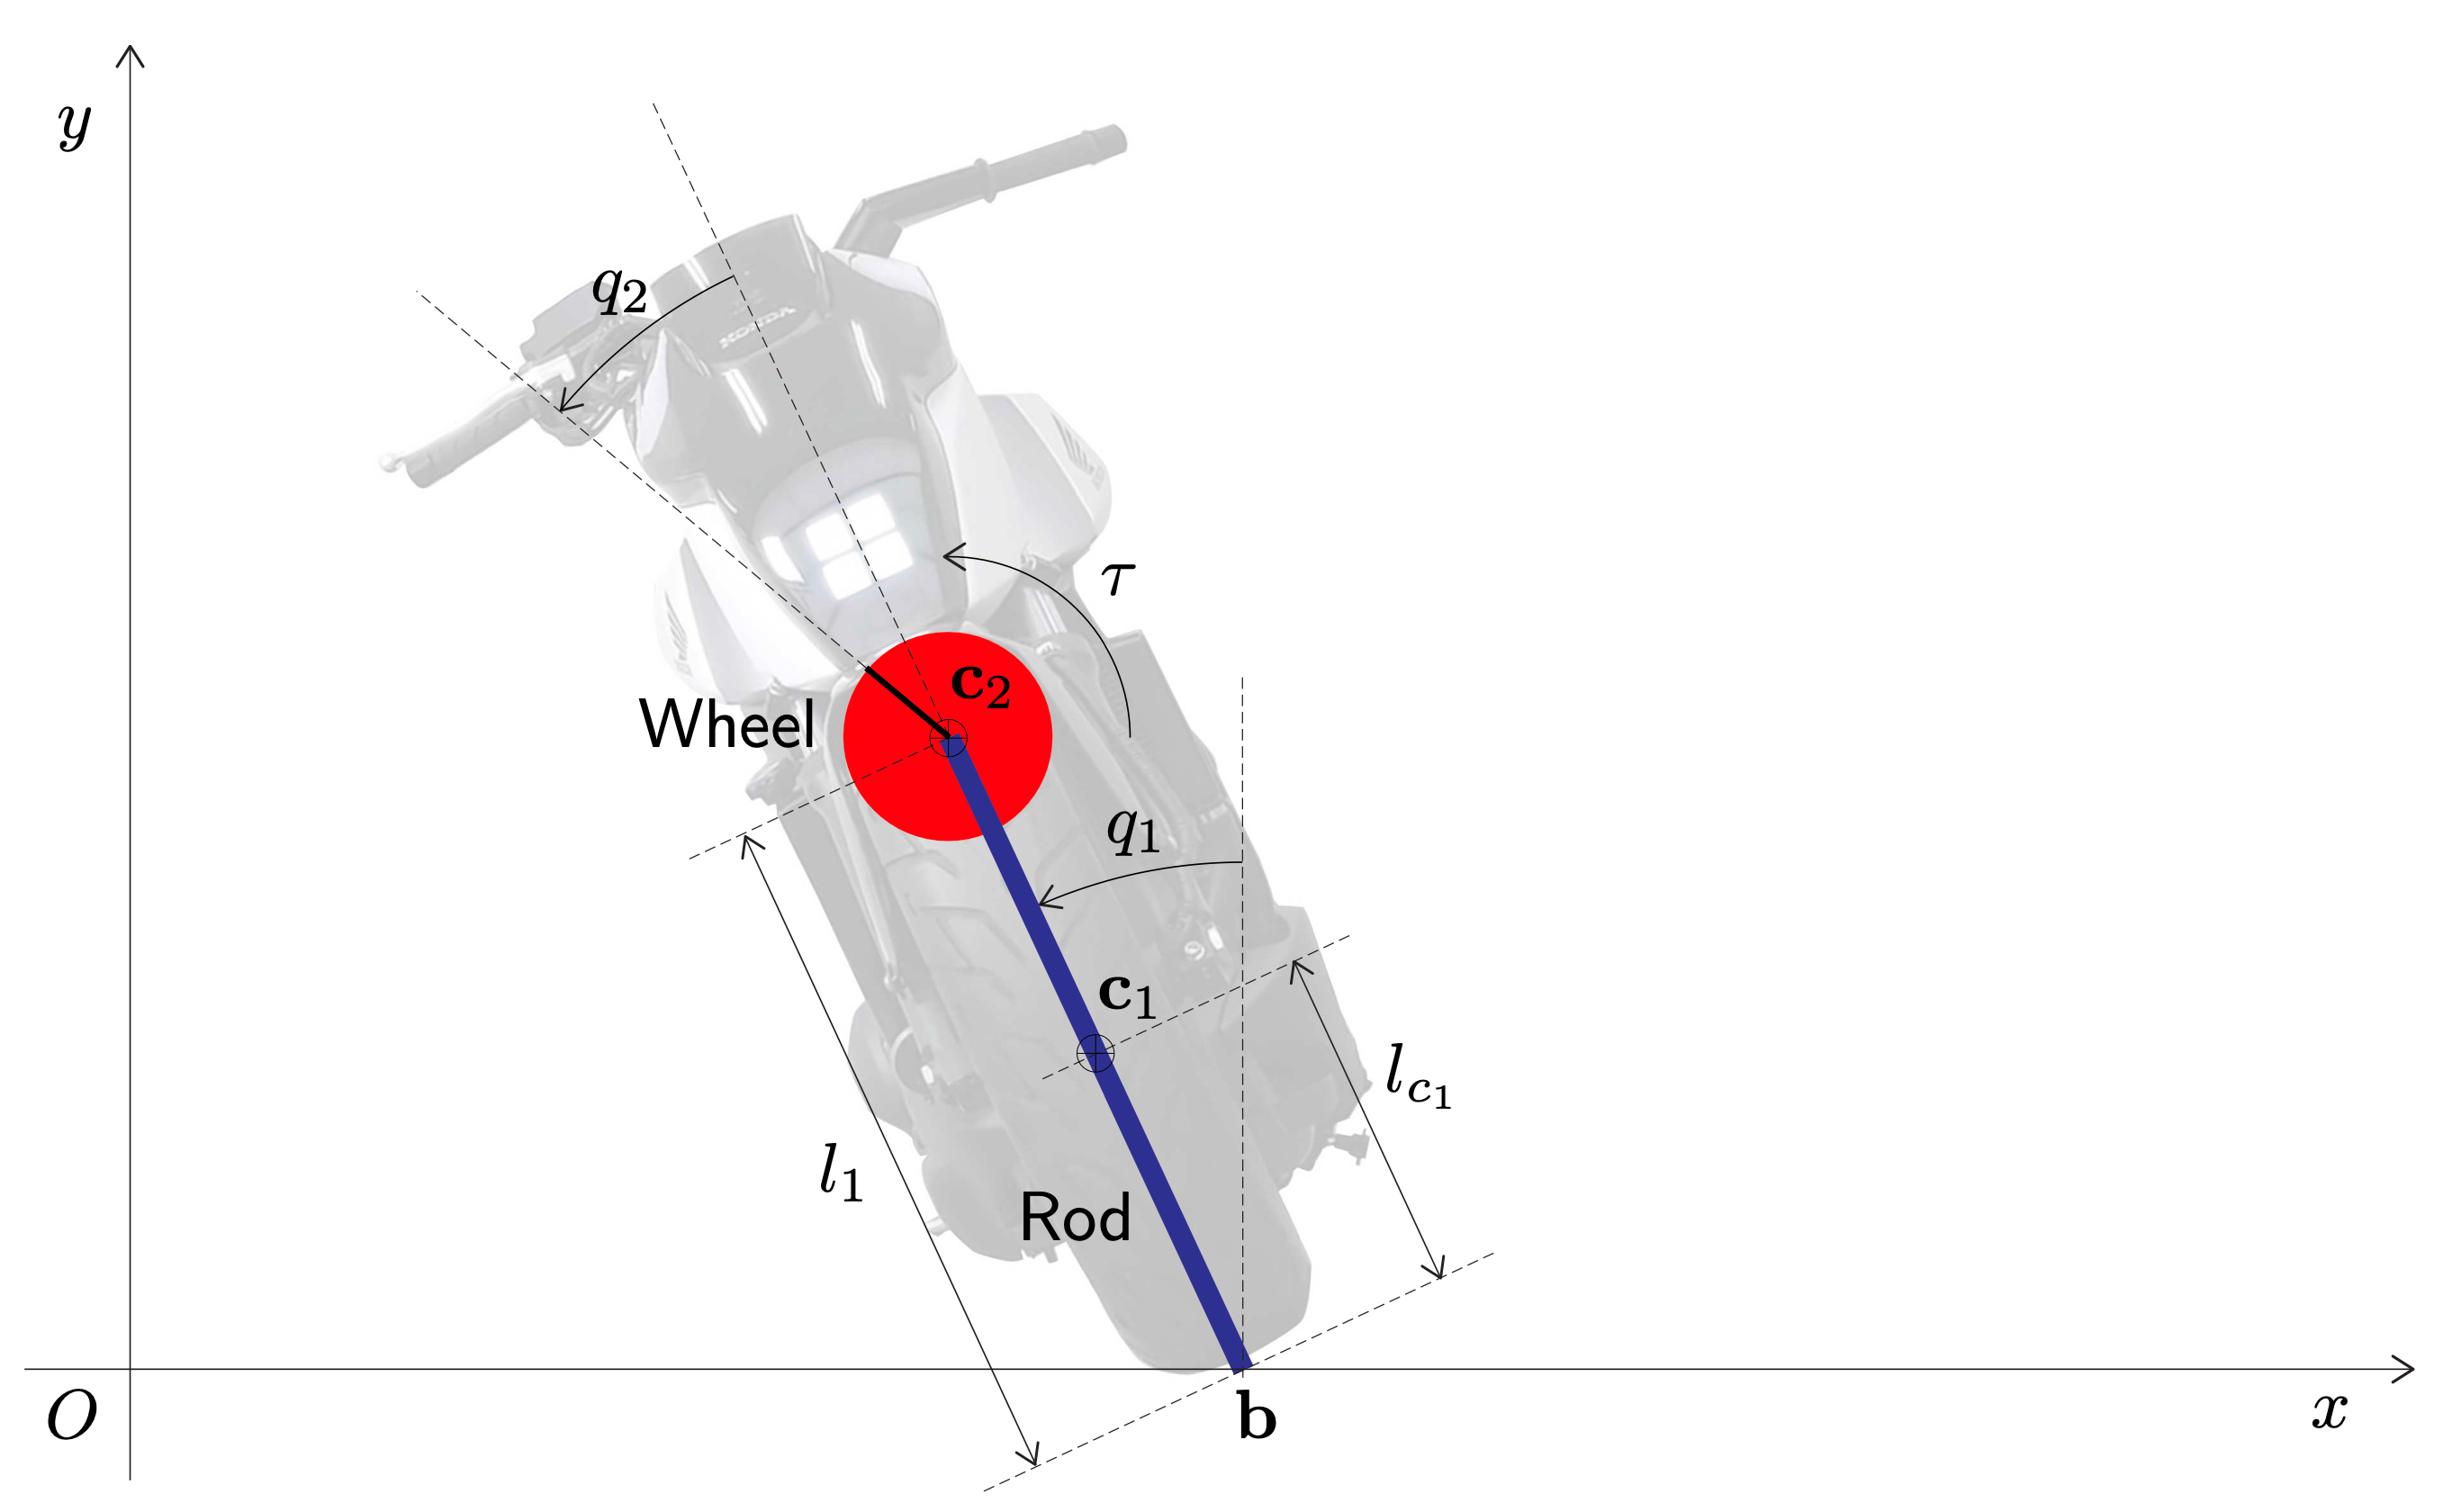
\includegraphics[width=1\linewidth]{figures/drawing}
\caption{Sketch of the control system for self balancing of a motorcycle}
\label{fig:figure_1}
\end{figure}




\noindent
The dynamic model of this system is
\begin{eqnarray*}
(m_1 l_{c_1}^2 + m_2 l_1^2 + I_1 + I_2) \ddot{q}_1 + I_2  \ddot{q}_2 - (m_1 l_{c_1} + m_2 l_1) g \sin (q_1)&=& 0,\\
I_2  \ddot{q}_1 + I_2  \ddot{q}_2&=& \tau,
\end{eqnarray*}
with the following parameters 
\begin{itemize}

\item
mass of the motorcycle $m_1 = 200 \; [\text{kg}]$, 

\item
mass of the reaction wheel $m_2 = 50 \; [\text{kg}]$, 

\item
barycentric moment of inertia of the motorcycle $I_1 = 25 \; [\text{kg m}^2]$, 

\item
barycentric moment of inertia of the reaction wheel $I_2 = 5 \; [\text{kg m}^2]$, 

\item
length of the rod $l_1 = 1 \; [\text{m}]$, 

\item
$l_{c_1} = \frac{l_1}{2} = 0.5\; [\text{m}]$,

\item
gravity acceleration: $g = 9.81 \; [\text{m}/\text{s}^2]$.
\end{itemize}


















\begin{itemize}
\item[1)] Intentionally omitted. 

\item[2)] Calculate the state space representation of the system, assuming that $\mathbf{x}  = ( x_1, x_2, x_3, x_4)^T = (q_1, q_2, \dot{q}_1, \dot{q_2})^T$, where angles are expressed in [rad] and angular velocities in [rad/s]. (Contesta en el informe y sube el c\'odigo \texttt{Matlab} a Aula Virtual en el fichero \texttt{statespace.m})

\item[3)] Calculate all the operating points of the system and explain the obtained result. (Contesta en el informe y sube el c\'odigo \texttt{Matlab} a Aula Virtual en el fichero \texttt{equilibrium.m})

\item[4)] Find the operating point that corresponds to $\overline{x}_1 = 0, \overline{u} = 0$. Linearize the system around this operating point.
(Contesta en el informe y sube el c\'odigo \texttt{Matlab} a Aula Virtual en el fichero \texttt{linearization.m})

\item[5)] 
Is the linearized system controllable? 
(Contesta en el informe y sube el c\'odigo \texttt{Matlab} a Aula Virtual en el fichero \texttt{controllability.m})

\item[6)] Is the linearized system observable by means of the output $y=x_1$? Is the linearized system controllable by means of the output $y = x_2$? (Contesta en el informe y sube el c\'odigo \texttt{Matlab} a Aula Virtual en el fichero \texttt{observability.m})


\item[7)] Using the pole placement method and an observer, design an output feedback controller to control the inclination of the motorcycle. 
We want to steer the motorcycle from the state $\mathbf{x} = (q_1, q_2, \dot{q}_1, \dot{q}_2)^T = (0.26179\if9387799149\fi,0,0,0)^T$ to the state $\mathbf{x} = (0, 0, 0, 0)^T$. 
Give the eigenvalues that have been assigned to the controlled system and illustrate the behaviour of the controller by plotting the relevant state and control variables and by a graphical animation. (Contesta en el informe y sube el c\'odigo \texttt{Matlab} a Aula Virtual en la carpeta \texttt{controller})


  

\end{itemize}

\bigskip

\noindent
\textcolor{red}{
Originality and completeness of the written answers will be the aspects that will be taken into account in the grading of the exam, and therefore, the \texttt{Matlab} code alone will not be considered. 
} 


\newpage

\section*{Solution}


\begin{itemize}

\item[2)] {\color{gray}  Calculate the state space representation of the system, assuming that $\mathbf{x}  = ( x_1, x_2, x_3, x_4)^T = (q_1, q_2, \dot{q}_1, \dot{q_2})^T$, where angles are expressed in [rad] and angular velocities in [rad/s]. (Contesta en el informe y sube el c\'odigo \texttt{Matlab} a Aula Virtual en el fichero \texttt{statespace.m})}

\bigskip

Para calcular las ecuaciones del espacio de estados se utiliza la función \textit{solve()} de MATLAB. Para luego poder decidir si sustituir o no, las variables g, m1, m2, l1, etc.se utilizan de forma simbólica. Por último lo único a tener en cuenta es que \textit{u} es igual a $\tau$.

\bigskip

\begin{tcolorbox}[width=12cm, title={File \texttt{statespace.m}}]
\begin{scriptsize}
\begin{verbatim}

close all
clc
clear

syms q1 q1dot q1ddot q2 q2dot q2ddot tao m1 m2 I1 I2 l1 lc1 g u;

% Known variables
% m1 = 200;
% m2 = 50;
% I1 = 25;
% I2 = 5;
% l1 = 1;
% lc1 = 0.5;
% g = 9.81;
tao = u

% State space representation x = [q1, q2, q1dot, q2dot];

% Define the dynamic equations
ecuaciones = [((m1*lc1^2 + m2*l1^2 + I1 + I2)*q1ddot + I2*q2ddot -(m1*lc1 +m2*l1)*g*sin(q1)==0),
(I2*q1ddot + I2*q2ddot - tao ==0)];
% Solve q1ddot and q2ddot
[q1ddot, q2ddot] = solve (ecuaciones,[q1ddot, q2ddot]);

% State representation
xdot = [q1dot; q2dot; q1ddot; q2ddot]

\end{verbatim}
\end{scriptsize}
\end{tcolorbox}

\item[3)]  {\color{gray} Calculate all the operating points of the system and explain the obtained result. (Contesta en el informe y sube el c\'odigo \texttt{Matlab} a Aula Virtual en el fichero \texttt{equilibrium.m})}

\bigskip

Para calcular los puntos operativos del sistema, se tiene que usar las ecuaciones del espacio de estados calculadas anteriormente. Para utilizarlas las definimos en \textit{f1, f2, f3 y f4} , que luego añadimos a la matriz \textit{eqs}, igualando todas las ecuaciones del espacio de estados a 0 para así encontrar los puntos operativos.\\
Se vuelve a usar otra vez la función \textit{solve()} de MATLAB, para las variables del espacio de estados (\textit{x1, x2, x3, x4 y u}) y con las todas las variables símbolicas usadas anteriormente sustituidas por sus valores reales, para así tener unos puntos operativos más exactos.\\
El resultado resultante, indica que el estado estará en equilibrio cuando ambas velocidades sean 0, es decir, $q{3}$ y $q{4}$ como son $\dot{q{1}]}=q{3}$ y $\dot{q{2}]}=q{2}$ respectivamente, derivadas del espacio. En cuanto a $u$, esta será 0. Luego $q{1}$, posición angular del péndulo, será $k·\pi$, siendo $k=1,2,3,....$ , es decir, el estado de equilibrio ocurrirá cuando el péndulo se encuentre totalmente hacia arriba o hacia abajo, sin ninguna velocidad, y además como $q{2}=x$ esto indica que da igual la posición en la que se encuentre la rueda respecto a su eje.

\bigskip

\begin{tcolorbox}[width=12cm, title={File \texttt{equilibrium.m}}]
\begin{scriptsize}
\begin{verbatim}

close all
clc
clear

syms x1 x2 x3 x4 tao m1 m2 I1 I2 l1 lc1 g u;

% Known variables
m1 = 200;
m2 = 50;
I1 = 25;
I2 = 5;
l1 = 1;
lc1 = 0.5;
g = 9.81;
tao = u;

f1 = x3;
f2 = x4;
f3 = (g*l1*m2*sin(x1) - tao + g*lc1*m1*sin(x1))/(m2*l1^2 + m1*lc1^2 + I1);
f4 = (m2*tao*l1^2 - I2*g*m2*sin(x1)*l1 + m1*tao*lc1^2 - I2*g*m1*sin(x1)*lc1 + I1*tao + I2*tao)/(I2*(m2*l1^2 + m1*lc1^2 + I1));

% Estado de equilibrio
eqs = [f1 == 0; f2 == 0; f3 == 0; f4 == 0 ];
S = solve(eqs, [x1, x2, x3, x4, u], 'ReturnConditions', true, 'Real', true);

q1 = S.x1
q2 = S.x2
q3 = S.x3
q4 = S.x4
barrau = S.u

\end{verbatim}
\end{scriptsize}
\end{tcolorbox}

\item[4)]  {\color{gray} Find the operating point that corresponds to $\overline{x}_1 = 0, \overline{u} = 0$. Linearize the system around this operating point.
(Contesta en el informe y sube el c\'odigo \texttt{Matlab} a Aula Virtual en el fichero \texttt{linearization.m})}

\bigskip

Con el resultado del apartado anterior se sabe que hay un punto operativo en $\overline{x}_1 = 0, \overline{u} = 0$, luego usando las ecuaciones del espacio de estados podemos calcular las matrices A, B, C y D, y en este caso podemos que suponer que $y=x{2}$ aunque esto no vaya a importar en los siguientes pasos.\\
Para conseguir las matrices anteriores se usa la función \textit{jacobian()} de MATLAB, y luego se usa otra función de MATLAB, \textit{subs()}, para substituir los valores que ya sabemos que son 0, como $x{1}, x{3}, x{4}, u$.\\
Hay que recordar que volvemos a dejar todas las constantes de forma simbólica para poder sustituirlas más adelante.

\bigskip

\begin{tcolorbox}[width=12cm, title={File \texttt{linearization.m}}]
\begin{scriptsize}
\begin{verbatim}

close all
clc
clear

syms x1 x2 x3 x4 tao m1 m2 I1 I2 l1 lc1 g u;

% Known variables
% m1 = 200;
% m2 = 50;
% I1 = 25;
% I2 = 5;
% l1 = 1;
% lc1 = 0.5;
% g = 9.81;
tao = u;

f1 = x3;
f2 = x4;
f3 = (g*l1*m2*sin(x1) - tao + g*lc1*m1*sin(x1))/(m2*l1^2 + m1*lc1^2 + I1);
f4 = (m2*tao*l1^2 - I2*g*m2*sin(x1)*l1 + m1*tao*lc1^2 - I2*g*m1*sin(x1)*lc1 + I1*tao + I2*tao)/(I2*(m2*l1^2 + m1*lc1^2 + I1));

% Estado de equilibrio
eqs = [f1; f2; f3; f4];
y = x2

A = jacobian(eqs,[x1, x2, x3, x4])
B = jacobian(eqs, u)
C = jacobian(y, [x1, x2, x3, x4])
D = jacobian(y, u)

Aeq = subs(A, [x1,x3,x4,u], [0,0,0,0])
eig(Aeq)
Beq = subs(B, [x1,x3,x4,u], [0,0,0,0])
Ceq = subs(C, [x1,x3,x4,u], [0,0,0,0])

\end{verbatim}
\end{scriptsize}
\end{tcolorbox}

\item[5)] 
 {\color{gray} Is the linearized system controllable? 
(Contesta en el informe y sube el c\'odigo \texttt{Matlab} a Aula Virtual en el fichero \texttt{controllability.m})}

\bigskip

Usando las matrices Aeq y Beq, que son A y B después de realizar la substitución, calculamos la matriz de controlabilidad usando la función \textit{crtb()} de MATLAB y observando su rango.\\
Como el rango resultante es 4, que coincide con el rango máximo de las ecuaciones de estado, se puede decir que el sistema es controlable en $\overline{x}_1 = 0, \overline{u} = 0$.

\bigskip

\begin{tcolorbox}[width=12cm, title={File \texttt{controllability.m}}]
\begin{scriptsize}
\begin{verbatim}

close all
clc
clear

syms x1 x2 x3 x4 tao m1 m2 I1 I2 l1 lc1 g u;

% Known variables
m1 = 200;
m2 = 50;
I1 = 25;
I2 = 5;
l1 = 1;
lc1 = 0.5;
g = 9.81;
tao = u;

f1 = x3;
f2 = x4;
f3 = (g*l1*m2*sin(x1) - tao + g*lc1*m1*sin(x1))/(m2*l1^2 + m1*lc1^2 + I1);
f4 = (m2*tao*l1^2 - I2*g*m2*sin(x1)*l1 + m1*tao*lc1^2 - I2*g*m1*sin(x1)*lc1 + I1*tao + I2*tao)/(I2*(m2*l1^2 + m1*lc1^2 + I1));

% Estado de equilibrio
eqs = [f1; f2; f3; f4];

A = jacobian(eqs,[x1, x2, x3, x4])
B = jacobian(eqs, u);

Aeq = subs(A, [x1,x3,x4,u], [0,0,0,0]);
Beq = subs(B, [x1,x3,x4,u], [0,0,0,0]);

eig(Aeq)

Co = ctrb(Aeq, Beq) 
rangoContrl = rank(Co) % Como el rango es maximo en 4 entonces es controlable

\end{verbatim}
\end{scriptsize}
\end{tcolorbox}

\item[6)]  {\color{gray} Is the linearized system observable by means of the output $y=x_1$? Is the linearized system observable by means of the output $y = x_2$? (Contesta en el informe y sube el c\'odigo \texttt{Matlab} a Aula Virtual en el fichero \texttt{observability.m})}

\bigskip

Aquí se repiten los mismos pasos que en apartado 4, ya que se necesita linearizar el sistema para $y=x{1}$ e $y=x{2}$. A los pasos seguidos en ese apartado hay que añadir el propio de la observabilidad, que es el cálculo de la matriz del mismo nombre y el estudio de su rango.\\
Si el rango de la matriz de observabilidad es igual al del rango máximo de las ecuaciones de estado, es decir, 4, entonces es observable.\\
Esto solo se cumple cuando $y=x{2}$, ya que cuando $y=x{1}$ el rango de la matriz resultante es 2, que es menor que el rango máximo.

\bigskip

\begin{tcolorbox}[width=12cm, title={File \texttt{observability.m}}]
\begin{scriptsize}
\begin{verbatim}

close all
clc
clear

syms x1 x2 x3 x4 tao m1 m2 I1 I2 l1 lc1 g u;

% Known variables
m1 = 200;
m2 = 50;
I1 = 25;
I2 = 5;
l1 = 1;
lc1 = 0.5;
g = 9.81;
tao = u;

f1 = x3;
f2 = x4;
f3 = (g*l1*m2*sin(x1) - tao + g*lc1*m1*sin(x1))/(m2*l1^2 + m1*lc1^2 + I1);
f4 = (m2*tao*l1^2 - I2*g*m2*sin(x1)*l1 + m1*tao*lc1^2 - I2*g*m1*sin(x1)*lc1 + I1*tao + I2*tao)/(I2*(m2*l1^2 + m1*lc1^2 + I1));

% Estado de equilibrio
eqs = [f1; f2; f3; f4];
y = x1;

A = jacobian(eqs,[x1, x2, x3, x4]);
B = jacobian(eqs, u);
C = jacobian(y, [x1, x2, x3, x4]);
D = jacobian(y, u);

Aeq = subs(A, [x1,x3,x4,u], [0,0,0,0]);
Beq = subs(B, [x1,x3,x4,u], [0,0,0,0]);
Ceq = subs(C, [x1,x3,x4,u], [0,0,0,0]);

Ob = obsv(Aeq, Ceq)
rangoObsv = rank(Ob) % Como el rango es 2 y el maximo es 4 entonces no es observable

y = x2;

A = jacobian(eqs,[x1, x2, x3, x4]);
B = jacobian(eqs, u);
C = jacobian(y, [x1, x2, x3, x4]);
D = jacobian(y, u);

Aeq = subs(A, [x1,x3,x4,u], [0,0,0,0]);
Beq = subs(B, [x1,x3,x4,u], [0,0,0,0]);
Ceq = subs(C, [x1,x3,x4,u], [0,0,0,0]);

Ob = obsv(Aeq, Ceq)
rangoObsv = rank(Ob) % Como el rango es maximo en 4 entonces es observable

\end{verbatim}
\end{scriptsize}
\end{tcolorbox}

\item[7)]  {\color{gray} Using the pole placement method and an observer, design an output feedback controller to control the inclination of the motorcycle. 
We want to steer the motorcycle from the state $\mathbf{x} = (q_1, q_2, \dot{q}_1, \dot{q}_2)^T = (0.26179\if9387799149\fi,0,0,0)^T$ to the state $\mathbf{x} = (0, 0, 0, 0)^T$. 
Give the eigenvalues that have been assigned to the controlled system and illustrate the behaviour of the controller by plotting the relevant state and control variables and by a graphical animation. (Contesta en el informe y sube el c\'odigo \texttt{Matlab} a Aula Virtual en la carpeta \texttt{controller})}

\bigskip

Se usa la estructura de código que se ha usado en clase para sistemas con observador, como por ejemplo el ejercicio 6.6, y se modifican las partes correspondientes a este sistema, como son la función $xdot()$ del fichero prac2\_f.m (en el que se usan las ecuaciones del espacio de estados obtenidas en el apartado 2), la función $xhatdot()$ del fichero prac2\_obs\_f.m (en el que usando las matrices obtenidas al linearizar en el apartado 4 para poder calcular $\dot{\hat{x}})$ como se explicará más adelante) y el \textit{main} del fichero prac2\_main.m. También se ha modificado la función \textit{draw} para poder realizar una representación adecuada del sistema.\\
Para todo esto se ha necesitado del cálculo de 3 matrices K, H y L usadas para obtener u y $\hat{x}$. La matriz K y L se obtienen usando la función \textit{place()} de MATLAB con las matrices calculadas en el apartado 4, es decir, A, B y C, y además con los polos del sistemas que hemos puesto de forma arbitraria en -2 tanto para el controlador como para el observador, ya que este valor da un control rápido, aunque se puede usar un valor menor para un control menos brusco, o uno mayor para el resultado contrario. (Recordar que para poner polos múltiples en MATLAB hay que ponerlos un poco separados unos de otros). Luego para extraer la matriz H se usan las matrices A, B, K y una nueva matriz fila $E = [0,1,0,0]$.\\
Con todo esto ya se obtiene la representación gráfica del control, pero cabe recordar que el estado inicial es el indicado en la pregunta $x = (0.26179\if9387799149\fi,0,0,0)^T$ tanto para x como para $\hat{x}$ del observador.

\begin{center}
	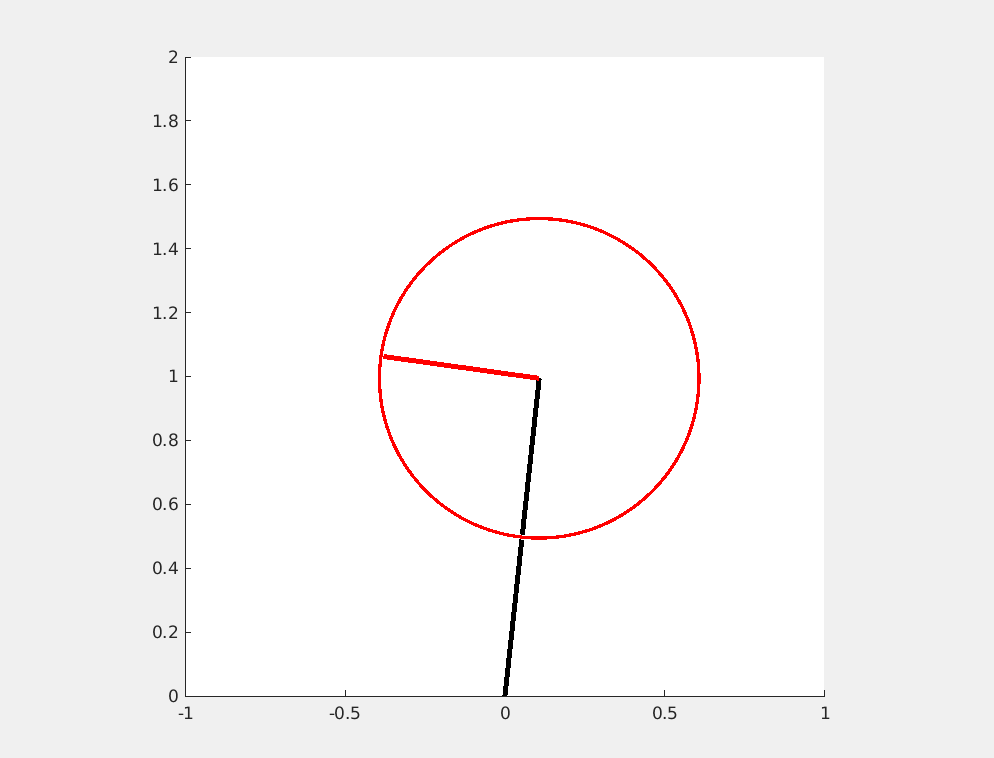
\includegraphics[width=0.9\textwidth]{figures/p2}
\end{center}

\bigskip
  

\end{itemize}




%\begin{tcolorbox}[width=12cm, title={File \texttt{file\_name.m}}]
%\begin{scriptsize}
%\begin{verbatim}
%
%
%\end{verbatim}
%\end{scriptsize}
%\end{tcolorbox}




%
%\begin{figure}[H]
%%\psfrag{m}{$a$}
%%\centerline{\includegraphics[width=0.75\columnwidth]{figures/figure_1.eps}}
%\caption{My caption.}
%\label{fig:figure_1}
%\end{figure}









\end{document}
